\chapter{Kiểm thử}

Chương này trình bày quá trình kiểm thử hệ thống Social Commerce sau giai đoạn hiện thực. Mục tiêu của kiểm thử là xác nhận các chức năng chính hoạt động đúng theo yêu cầu, API trả về dữ liệu nhất quán, các luồng phân quyền được bảo vệ hợp lý và giao diện người dùng đạt mức phản hồi chấp nhận được trong môi trường kiểm thử.

Phạm vi kiểm thử tập trung vào ba nhóm chính:

\begin{itemize}
    \item Kiểm thử API bằng Postman đối với core API và admin API.
    \item Kiểm thử luồng chức năng thông qua các kịch bản người dùng (user), seller và admin.
    \item Kiểm thử hiệu suất giao diện bằng Chrome DevTools và Lighthouse.
\end{itemize}

\section{Công cụ kiểm thử}

\subsection{Công cụ hỗ trợ kiểm thử Postman}

Postman được sử dụng làm công cụ chính để kiểm thử API vì phù hợp với hệ thống backend được xây dựng theo mô hình REST API. Công cụ này hỗ trợ tạo collection endpoint, cấu hình biến môi trường, lưu token sau khi đăng nhập và kiểm tra response tự động bằng script.

Trong quá trình kiểm thử, nhóm cấu hình các biến môi trường chính như sau:

\begin{table}[H]
\centering
\caption{Các biến môi trường sử dụng trong Postman}
\begin{tabularx}{\textwidth}{|p{0.28\textwidth}|X|}
\hline
\textbf{Biến môi trường} & \textbf{Ý nghĩa} \\ \hline
\texttt{baseUrl} & URL của core backend API, ví dụ \texttt{http://localhost:5000/api}. \\ \hline
\texttt{adminBaseUrl} & URL của admin backend API, ví dụ \texttt{http://localhost:5001/api}. \\ \hline
\texttt{accessToken} & JWT token của buyer/seller sau khi đăng nhập thành công. \\ \hline
\texttt{adminToken} & JWT token của admin sau khi đăng nhập admin. \\ \hline
\texttt{userId}, \texttt{productId}, \texttt{postId}, \texttt{orderId} & Các ID được lấy từ response trước đó để dùng cho các request phụ thuộc. \\ \hline
\end{tabularx}
\end{table}

Các nhóm API được đưa vào Postman collection gồm:

\begin{itemize}
    \item \textbf{Authentication}: đăng ký, xác thực email, đăng nhập, đăng xuất, quên mật khẩu, reset password và 2FA.
    \item \textbf{User/Profile}: xem và cập nhật hồ sơ, follow/unfollow, tìm kiếm người dùng.
    \item \textbf{Social}: bài viết, feed, like, comment, saved items, báo cáo vi phạm.
    \item \textbf{Commerce}: sản phẩm, danh mục, giỏ hàng, checkout, đơn hàng và đánh giá.
    \item \textbf{Seller}: đăng ký seller, trạng thái hồ sơ, sản phẩm seller, biến thể sản phẩm và đơn bán.
    \item \textbf{Messaging/Notification}: conversation, message, notification và notification preferences.
    \item \textbf{AI/Scheduled posts}: tạo nội dung AI, lưu lịch sử AI, tư vấn mua sắm qua AI chatbox, tạo và quản lý bài viết đã lên lịch.
    \item \textbf{Admin}: đăng nhập admin, dashboard, users, posts, products, reports, seller applications và sensitive change requests.
\end{itemize}

\section{Kiểm thử API}

\subsection{Cách thực hiện}

Quy trình kiểm thử API được thực hiện theo các bước sau:

\begin{enumerate}
    \item \textbf{Chuẩn bị dữ liệu}: tạo các tài khoản kiểm thử gồm buyer, seller và admin; seed dữ liệu sản phẩm, bài viết, danh mục, đơn hàng và báo cáo vi phạm.
    \item \textbf{Đăng nhập và lưu token}: gọi API đăng nhập, lưu JWT vào biến môi trường Postman để dùng cho các request yêu cầu xác thực.
    \item \textbf{Kiểm thử request hợp lệ}: gửi request với dữ liệu đúng và kiểm tra HTTP status code, cấu trúc response, message và dữ liệu trả về.
    \item \textbf{Kiểm thử request không hợp lệ}: gửi dữ liệu thiếu field, sai định dạng, token không hợp lệ hoặc sai role để kiểm tra validation và authorization.
    \item \textbf{Kiểm thử dữ liệu phụ thuộc}: với các luồng như tạo sản phẩm, thêm giỏ hàng, checkout, tạo review, nhóm kiểm tra thứ tự request và dữ liệu sinh ra từ bước trước.
    \item \textbf{Đối chiếu database}: với các chức năng ghi dữ liệu quan trọng, kiểm tra lại dữ liệu trong PostgreSQL thông qua Prisma Studio hoặc database client.
    \item \textbf{Kiểm tra side effect}: xác nhận các side effect như tăng số lượng like/comment, tạo notification, cập nhật trạng thái đơn hàng hoặc lưu lịch sử AI.
\end{enumerate}

Các tiêu chí đánh giá kết quả gồm:

\begin{itemize}
    \item API trả đúng status code: \texttt{200}, \texttt{201}, \texttt{400}, \texttt{401}, \texttt{403}, \texttt{404} tùy tình huống.
    \item Response có cấu trúc thống nhất, thường gồm \texttt{success}, \texttt{message}, \texttt{data} và \texttt{pagination} nếu là danh sách.
    \item Các endpoint yêu cầu đăng nhập phải từ chối request không có token hoặc token sai.
    \item Các endpoint dành cho seller/admin phải kiểm tra đúng quyền truy cập.
    \item Dữ liệu tạo mới/cập nhật/xóa mềm phải phản ánh đúng trong database.
\end{itemize}

\subsection{Kết quả test case tổng hợp}

Bảng sau tổng hợp kết quả kiểm thử theo từng nhóm chức năng chính của hệ thống.

\begin{longtable}{|>{\raggedright\arraybackslash}p{0.15\textwidth}|p{0.24\textwidth}|p{0.36\textwidth}|p{0.14\textwidth}|}
\caption{Kết quả kiểm thử API tổng hợp} \\
\hline
\textbf{Mã nhóm} & \textbf{Nhóm chức năng} & \textbf{Nội dung kiểm thử chính} & \textbf{Kết quả} \\ \hline
\endfirsthead
\hline
\textbf{Mã nhóm} & \textbf{Nhóm chức năng} & \textbf{Nội dung kiểm thử chính} & \textbf{Kết quả} \\ \hline
\endhead
AUTH & Xác thực tài khoản & Đăng ký, xác thực email, đăng nhập, đăng xuất, quên mật khẩu, reset password, bật/tắt 2FA. & Đạt \\ \hline
USER & Hồ sơ và quan hệ người dùng & Xem/cập nhật hồ sơ, tìm kiếm user, follow/unfollow, quyền truy cập hồ sơ. & Đạt \\ \hline
POST & Bài viết và feed & Tạo bài viết, gắn nhiều sản phẩm qua \texttt{productTags}, xem feed, like, comment, share, xóa bài viết. & Đạt \\ \hline
GROUP & Nhóm cộng đồng & Tạo nhóm, tham gia/rời nhóm, duyệt yêu cầu tham gia, bài viết trong nhóm, invite. & Đạt \\ \hline
PRODUCT & Sản phẩm và marketplace & Tạo/sửa/xóa mềm/khôi phục sản phẩm, ảnh sản phẩm, biến thể, danh mục, tìm kiếm và lọc sản phẩm. & Đạt \\ \hline
CART & Giỏ hàng & Thêm sản phẩm vào giỏ, cập nhật số lượng, xóa item, lấy tổng số item. & Đạt \\ \hline
ORDER & Đơn hàng & Checkout, xem đơn mua/bán, cập nhật trạng thái, hủy đơn, yêu cầu hoàn tiền giả lập. & Đạt \\ \hline
REVIEW & Đánh giá sản phẩm & Tạo review sau mua, xem review, seller phản hồi review. & Đạt \\ \hline
MSG & Tin nhắn và thông báo & Tạo conversation, gửi tin nhắn, đánh dấu đã đọc, lấy notification, cập nhật preferences. & Đạt \\ \hline
AI & AI, chatbox và bài lên lịch & Tạo text/image content, lưu AI history, tư vấn mua sắm qua AI chatbox, tạo/sửa/xóa/publish scheduled post. & Đạt \\ \hline
REPORT & Báo cáo vi phạm & Buyer/seller tạo report cho post, comment, product, user; admin xem và xử lý report. & Đạt \\ \hline
ADMIN & Quản trị hệ thống & Đăng nhập admin, dashboard, quản lý users, posts, products, categories, seller applications. & Đạt \\ \hline
\end{longtable}

\subsection{Kịch bản và kết quả kiểm thử}

Phần này mô tả các kịch bản kiểm thử tiêu biểu đã được thực hiện trên Postman và giao diện web. Các kịch bản được chọn để bao phủ các luồng nghiệp vụ quan trọng và các trường hợp phân quyền thường gặp.

\newcommand{\apiendpoint}[1]{\begingroup\ttfamily\scriptsize\seqsplit{#1}\endgroup}
{\scriptsize
\setlength{\tabcolsep}{1.5pt}
\renewcommand{\arraystretch}{1.12}
\begin{longtable}{|>{\centering\arraybackslash}p{0.045\textwidth}|>{\raggedright\arraybackslash}p{0.09\textwidth}|>{\raggedright\arraybackslash}p{0.20\textwidth}|>{\raggedright\arraybackslash}p{0.22\textwidth}|>{\raggedright\arraybackslash}p{0.325\textwidth}|>{\centering\arraybackslash}p{0.055\textwidth}|}
\caption{Kịch bản kiểm thử chức năng và API chi tiết} \\
\hline
\textbf{STT} & \textbf{Nhóm API} & \textbf{Tên API} & \textbf{Testcase thực hiện} & \textbf{Kết quả mong muốn} & \textbf{Kết quả} \\ \hline
\endfirsthead
\hline
\textbf{STT} & \textbf{Nhóm API} & \textbf{Tên API} & \textbf{Testcase thực hiện} & \textbf{Kết quả mong muốn} & \textbf{Kết quả} \\ \hline
\endhead
1 & auth & \apiendpoint{POST /api/auth/register} & \texttt{TC\_AUTH\_01} - Register success for buyer & Status code \texttt{201}; response có \texttt{success=true}; user được tạo ở trạng thái chờ xác thực email. & PASS \\ \hline
2 & auth & \apiendpoint{POST /api/auth/register} & \texttt{TC\_AUTH\_02} - Register success for seller account & Status code \texttt{201}; user được tạo với role phù hợp; gửi OTP xác thực email. & PASS \\ \hline
3 & auth & \apiendpoint{POST /api/auth/register} & \texttt{TC\_AUTH\_03} - Register fail duplicate email & Status code \texttt{400}/\texttt{409}; message thông báo email đã được sử dụng. & PASS \\ \hline
4 & auth & \apiendpoint{POST /api/auth/register} & \texttt{TC\_AUTH\_04} - Register fail duplicate username & Status code \texttt{400}/\texttt{409}; message thông báo username đã được sử dụng. & PASS \\ \hline
5 & auth & \apiendpoint{POST /api/auth/register} & \texttt{TC\_AUTH\_05} - Register fail missing required fields & Status code \texttt{400}; response có validation error; không tạo user. & PASS \\ \hline
6 & auth & \apiendpoint{POST /api/auth/register} & \texttt{TC\_AUTH\_06} - Register fail weak password & Status code \texttt{400}; message yêu cầu password hợp lệ. & PASS \\ \hline
7 & auth & \apiendpoint{POST /api/auth/verify-email} & \texttt{TC\_AUTH\_07} - Verify email success & Status code \texttt{200}; user chuyển sang trạng thái verified. & PASS \\ \hline
8 & auth & \apiendpoint{POST /api/auth/verify-email} & \texttt{TC\_AUTH\_08} - Verify email fail invalid OTP & Status code \texttt{400}; không xác thực tài khoản. & PASS \\ \hline
9 & auth & \apiendpoint{POST /api/auth/resend-verification} & \texttt{TC\_AUTH\_09} - Resend verification success & Status code \texttt{200}; hệ thống gửi lại OTP xác thực email. & PASS \\ \hline
10 & auth & \apiendpoint{POST /api/auth/login} & \texttt{TC\_AUTH\_10} - Login success for buyer & Status code \texttt{200}; trả access token và thông tin buyer. & PASS \\ \hline
11 & auth & \apiendpoint{POST /api/auth/login} & \texttt{TC\_AUTH\_11} - Login success for seller & Status code \texttt{200}; trả access token và thông tin seller. & PASS \\ \hline
12 & auth & \apiendpoint{POST /api/auth/login} & \texttt{TC\_AUTH\_12} - Login fail wrong password & Status code \texttt{401}; không trả token. & PASS \\ \hline
13 & auth & \apiendpoint{POST /api/auth/login} & \texttt{TC\_AUTH\_13} - Login fail unverified account & Status code \texttt{403}; response trả thông tin cần xác thực email. & PASS \\ \hline
14 & auth & \apiendpoint{POST /api/auth/login} & \texttt{TC\_AUTH\_14} - Login requires 2FA & Status code \texttt{200}; response có \texttt{requires2FA=true} và \texttt{tempToken}. & PASS \\ \hline
15 & auth & \apiendpoint{POST /api/auth/verify-2fa} & \texttt{TC\_AUTH\_15} - Verify 2FA success & Status code \texttt{200}; trả access token chính thức sau khi OTP đúng. & PASS \\ \hline
16 & auth & \apiendpoint{POST /api/auth/verify-2fa} & \texttt{TC\_AUTH\_16} - Verify 2FA fail wrong OTP & Status code \texttt{400}/\texttt{401}; không cấp access token. & PASS \\ \hline
17 & auth & \apiendpoint{GET /api/auth/me} & \texttt{TC\_AUTH\_17} - Get current user success & Status code \texttt{200}; response trả đúng user theo JWT. & PASS \\ \hline
18 & auth & \apiendpoint{GET /api/auth/me} & \texttt{TC\_AUTH\_18} - Get current user without token & Status code \texttt{401}; không trả thông tin user. & PASS \\ \hline
19 & auth & \apiendpoint{PUT /api/auth/profile} & \texttt{TC\_AUTH\_19} - Update profile success & Status code \texttt{200}; profile được cập nhật đúng dữ liệu gửi lên. & PASS \\ \hline
20 & auth & \apiendpoint{PUT /api/auth/password} & \texttt{TC\_AUTH\_20} - Change password success & Status code \texttt{200}; password mới dùng được khi đăng nhập lại. & PASS \\ \hline
21 & auth & \apiendpoint{PUT /api/auth/password} & \texttt{TC\_AUTH\_21} - Change password fail wrong current password & Status code \texttt{400}/\texttt{401}; password không bị thay đổi. & PASS \\ \hline
22 & auth & \apiendpoint{POST /api/auth/2fa/enable} & \texttt{TC\_AUTH\_22} - Enable 2FA send OTP & Status code \texttt{200}; OTP được gửi tới email. & PASS \\ \hline
23 & auth & \apiendpoint{POST /api/auth/2fa/confirm} & \texttt{TC\_AUTH\_23} - Confirm enable 2FA success & Status code \texttt{200}; \texttt{isEnabled=true}. & PASS \\ \hline
24 & auth & \apiendpoint{POST /api/auth/2fa/disable} & \texttt{TC\_AUTH\_24} - Disable 2FA success & Status code \texttt{200}; 2FA được tắt sau khi nhập đúng password. & PASS \\ \hline
25 & auth & \apiendpoint{POST /api/auth/2fa/disable} & \texttt{TC\_AUTH\_25} - Disable 2FA fail wrong password & Status code \texttt{400}/\texttt{401}; 2FA vẫn bật. & PASS \\ \hline

26 & user & \apiendpoint{GET /api/users/me} & \texttt{TC\_USER\_01} - Get my profile success & Status code \texttt{200}; trả profile của user hiện tại. & PASS \\ \hline
27 & user & \apiendpoint{PUT /api/users/me} & \texttt{TC\_USER\_02} - Update my profile success & Status code \texttt{200}; dữ liệu profile được cập nhật. & PASS \\ \hline
28 & user & \apiendpoint{GET /api/users/search} & \texttt{TC\_USER\_03} - Search users success & Status code \texttt{200}; response trả danh sách user phù hợp keyword. & PASS \\ \hline
29 & user & \apiendpoint{POST /api/users/:userId/follow} & \texttt{TC\_USER\_04} - Follow user success & Status code \texttt{200}; tạo quan hệ follow và notification. & PASS \\ \hline
30 & user & \apiendpoint{POST /api/users/:userId/follow} & \texttt{TC\_USER\_05} - Follow self fail & Status code \texttt{400}; không tạo quan hệ follow. & PASS \\ \hline
31 & user & \apiendpoint{DELETE /api/users/:userId/follow} & \texttt{TC\_USER\_06} - Unfollow success & Status code \texttt{200}; quan hệ follow bị xóa. & PASS \\ \hline
32 & user & \apiendpoint{GET /api/users/:userId} & \texttt{TC\_USER\_07} - Get public profile success & Status code \texttt{200}; trả public profile. & PASS \\ \hline
33 & user & \apiendpoint{GET /api/users/:userId} & \texttt{TC\_USER\_08} - Get nonexistent user & Status code \texttt{404}; response có message phù hợp. & PASS \\ \hline

34 & post & \apiendpoint{GET /api/posts} & \texttt{TC\_POST\_01} - Get public posts success & Status code \texttt{200}; response có data và pagination. & PASS \\ \hline
35 & post & \apiendpoint{GET /api/posts/feed} & \texttt{TC\_POST\_02} - Get personalized feed success & Status code \texttt{200}; trả feed theo user đã đăng nhập. & PASS \\ \hline
36 & post & \apiendpoint{GET /api/posts/feed} & \texttt{TC\_POST\_03} - Get feed without token & Status code \texttt{401}; không trả personalized feed. & PASS \\ \hline
37 & post & \apiendpoint{POST /api/posts} & \texttt{TC\_POST\_04} - Create post success & Status code \texttt{201}; bài viết được lưu vào database. & PASS \\ \hline
38 & post & \apiendpoint{POST /api/posts} & \texttt{TC\_POST\_05} - Create post with multiple product tags & Status code \texttt{201}; response có \texttt{taggedProducts}; tạo bản ghi \textit{post\_product\_tags}. & PASS \\ \hline
39 & post & \apiendpoint{POST /api/posts} & \texttt{TC\_POST\_06} - Create post fail invalid productTags & Status code \texttt{400}; không tạo bài viết/tag. & PASS \\ \hline
40 & post & \apiendpoint{PUT /api/posts/:id} & \texttt{TC\_POST\_07} - Update own post success & Status code \texttt{200}; nội dung bài viết được cập nhật. & PASS \\ \hline
41 & post & \apiendpoint{PUT /api/posts/:id} & \texttt{TC\_POST\_08} - Update another user's post fail & Status code \texttt{403}; bài viết không bị thay đổi. & PASS \\ \hline
42 & post & \apiendpoint{DELETE /api/posts/:id} & \texttt{TC\_POST\_09} - Delete own post success & Status code \texttt{200}; bài viết bị xóa/ẩn khỏi danh sách. & PASS \\ \hline
43 & post & \apiendpoint{GET /api/posts/:id} & \texttt{TC\_POST\_10} - Get nonexistent post & Status code \texttt{404}; message \texttt{Post not found}. & PASS \\ \hline
44 & post & \apiendpoint{POST /api/posts/:id/like} & \texttt{TC\_POST\_11} - Like/unlike success & Status code \texttt{200}; trạng thái like được toggle. & PASS \\ \hline
45 & post & \apiendpoint{POST /api/posts/:id/comments} & \texttt{TC\_POST\_12} - Add comment success & Status code \texttt{201}/\texttt{200}; comment được lưu. & PASS \\ \hline
46 & post & \apiendpoint{POST /api/posts/:id/comments} & \texttt{TC\_POST\_13} - Add empty comment fail & Status code \texttt{400}; không tạo comment. & PASS \\ \hline
47 & post & \apiendpoint{GET /api/posts/:id/comments} & \texttt{TC\_POST\_14} - Get comments success & Status code \texttt{200}; trả danh sách comment theo phân trang. & PASS \\ \hline

48 & product & \apiendpoint{GET /api/products} & \texttt{TC\_PROD\_01} - Get product list success & Status code \texttt{200}; response có data và pagination. & PASS \\ \hline
49 & product & \apiendpoint{GET /api/products?search=...} & \texttt{TC\_PROD\_02} - Search/filter products success & Status code \texttt{200}; danh sách phản ánh keyword/filter. & PASS \\ \hline
50 & product & \apiendpoint{GET /api/products/:id} & \texttt{TC\_PROD\_03} - Get product detail success & Status code \texttt{200}; trả thông tin sản phẩm, ảnh, variant, seller. & PASS \\ \hline
51 & product & \apiendpoint{GET /api/products/:id} & \texttt{TC\_PROD\_04} - Product not found & Status code \texttt{404}; message \texttt{Product not found}. & PASS \\ \hline
52 & product & \apiendpoint{POST /api/products} & \texttt{TC\_PROD\_05} - Seller create product success & Status code \texttt{201}; sản phẩm thuộc seller hiện tại. & PASS \\ \hline
53 & product & \apiendpoint{POST /api/products} & \texttt{TC\_PROD\_06} - Buyer create product fail & Status code \texttt{403}; không tạo sản phẩm. & PASS \\ \hline
54 & product & \apiendpoint{POST /api/products} & \texttt{TC\_PROD\_07} - Create product fail missing title/price & Status code \texttt{400}; validation error. & PASS \\ \hline
55 & product & \apiendpoint{PUT /api/products/:id} & \texttt{TC\_PROD\_08} - Seller update own product success & Status code \texttt{200}; sản phẩm được cập nhật. & PASS \\ \hline
56 & product & \apiendpoint{PUT /api/products/:id} & \texttt{TC\_PROD\_09} - Seller update other seller product fail & Status code \texttt{403}/\texttt{404}; không cập nhật dữ liệu. & PASS \\ \hline
57 & product & \apiendpoint{DELETE /api/products/:id} & \texttt{TC\_PROD\_10} - Soft delete product success & Status code \texttt{200}; sản phẩm chuyển trạng thái xóa mềm. & PASS \\ \hline
58 & product & \apiendpoint{POST /api/products/:id/restore} & \texttt{TC\_PROD\_11} - Restore product success & Status code \texttt{200}; sản phẩm được khôi phục. & PASS \\ \hline
59 & product & \apiendpoint{POST /api/products/:id/publish} & \texttt{TC\_PROD\_12} - Publish product success & Status code \texttt{200}; sản phẩm chuyển trạng thái hiển thị. & PASS \\ \hline
60 & product & \apiendpoint{POST /api/products/:id/images} & \texttt{TC\_PROD\_13} - Add images success & Status code \texttt{200}; ảnh sản phẩm được thêm. & PASS \\ \hline
61 & product & \apiendpoint{POST /api/products/:id/images} & \texttt{TC\_PROD\_14} - Add images fail invalid body & Status code \texttt{400}; không thêm ảnh. & PASS \\ \hline
62 & product & \apiendpoint{POST /api/products/seller/me/:productId/variants} & \texttt{TC\_PROD\_15} - Create variant success & Status code \texttt{201}/\texttt{200}; variant được tạo cho sản phẩm của seller. & PASS \\ \hline
63 & product & \apiendpoint{POST /api/products/seller/me/:productId/variants} & \texttt{TC\_PROD\_16} - Create variant fail invalid stock/price & Status code \texttt{400}; không tạo variant. & PASS \\ \hline

64 & cart & \apiendpoint{GET /api/cart} & \texttt{TC\_CART\_01} - Get cart success & Status code \texttt{200}; trả cart, items, subtotal. & PASS \\ \hline
65 & cart & \apiendpoint{GET /api/cart} & \texttt{TC\_CART\_02} - Get cart without token & Status code \texttt{401}; không trả cart. & PASS \\ \hline
66 & cart & \apiendpoint{POST /api/cart/items} & \texttt{TC\_CART\_03} - Add item success & Status code \texttt{201}/\texttt{200}; cart item được tạo/cập nhật. & PASS \\ \hline
67 & cart & \apiendpoint{POST /api/cart/items} & \texttt{TC\_CART\_04} - Add item fail quantity less than 1 & Status code \texttt{400}; cart không thay đổi. & PASS \\ \hline
68 & cart & \apiendpoint{POST /api/cart/items} & \texttt{TC\_CART\_05} - Add nonexistent product & Status code \texttt{404}; không tạo cart item. & PASS \\ \hline
69 & cart & \apiendpoint{PUT /api/cart/items/:itemId} & \texttt{TC\_CART\_06} - Update quantity success & Status code \texttt{200}; số lượng item được cập nhật. & PASS \\ \hline
70 & cart & \apiendpoint{PUT /api/cart/items/:itemId} & \texttt{TC\_CART\_07} - Update item not owned fail & Status code \texttt{403}; không cập nhật item. & PASS \\ \hline
71 & cart & \apiendpoint{DELETE /api/cart/items/:itemId} & \texttt{TC\_CART\_08} - Remove item success & Status code \texttt{200}; item bị xóa khỏi cart. & PASS \\ \hline
72 & cart & \apiendpoint{DELETE /api/cart} & \texttt{TC\_CART\_09} - Clear cart success & Status code \texttt{200}; cart không còn item. & PASS \\ \hline

73 & order & \apiendpoint{POST /api/orders} & \texttt{TC\_ORDER\_01} - Checkout success & Status code \texttt{201}; tạo order và order items. & PASS \\ \hline
74 & order & \apiendpoint{POST /api/orders} & \texttt{TC\_ORDER\_02} - Checkout fail empty cart & Status code \texttt{400}; không tạo order. & PASS \\ \hline
75 & order & \apiendpoint{POST /api/orders} & \texttt{TC\_ORDER\_03} - Checkout fail invalid shipping phone & Status code \texttt{400}; validation error. & PASS \\ \hline
76 & order & \apiendpoint{GET /api/orders/my/purchases} & \texttt{TC\_ORDER\_04} - Get buyer orders success & Status code \texttt{200}; trả danh sách đơn mua. & PASS \\ \hline
77 & order & \apiendpoint{GET /api/orders/my/sales} & \texttt{TC\_ORDER\_05} - Get seller sales success & Status code \texttt{200}; trả danh sách đơn bán liên quan seller. & PASS \\ \hline
78 & order & \apiendpoint{GET /api/orders/:orderId} & \texttt{TC\_ORDER\_06} - Get own order success & Status code \texttt{200}; trả chi tiết order. & PASS \\ \hline
79 & order & \apiendpoint{GET /api/orders/:orderId} & \texttt{TC\_ORDER\_07} - Get another user's order fail & Status code \texttt{403}; không lộ dữ liệu đơn hàng. & PASS \\ \hline
80 & order & \apiendpoint{PUT /api/orders/:orderId/status} & \texttt{TC\_ORDER\_08} - Seller update status success & Status code \texttt{200}; trạng thái đơn được cập nhật hợp lệ. & PASS \\ \hline
81 & order & \apiendpoint{PUT /api/orders/:orderId/status} & \texttt{TC\_ORDER\_09} - Invalid status transition fail & Status code \texttt{400}; trạng thái không đổi. & PASS \\ \hline
82 & order & \apiendpoint{POST /api/orders/:orderId/cancel} & \texttt{TC\_ORDER\_10} - Cancel pending order success & Status code \texttt{200}; order chuyển cancelled. & PASS \\ \hline
83 & order & \apiendpoint{POST /api/orders/:orderId/cancel} & \texttt{TC\_ORDER\_11} - Cancel delivered order fail & Status code \texttt{400}; order không bị hủy. & PASS \\ \hline
84 & order & \apiendpoint{POST /api/orders/:orderId/payment/confirm} & \texttt{TC\_ORDER\_12} - Confirm payment success & Status code \texttt{200}; paymentStatus được cập nhật. & PASS \\ \hline
85 & order & \apiendpoint{POST /api/orders/:orderId/refund-request} & \texttt{TC\_ORDER\_13} - Request refund success & Status code \texttt{200}; lưu yêu cầu hoàn tiền. & PASS \\ \hline
86 & order & \apiendpoint{POST /api/orders/:orderId/refund} & \texttt{TC\_ORDER\_14} - Seller process refund success & Status code \texttt{200}; trạng thái refund được xử lý. & PASS \\ \hline

87 & review & \apiendpoint{GET /api/reviews/product/:productId} & \texttt{TC\_REV\_01} - Get product reviews success & Status code \texttt{200}; trả danh sách review. & PASS \\ \hline
88 & review & \apiendpoint{POST /api/reviews} & \texttt{TC\_REV\_02} - Create review success & Status code \texttt{201}; review liên kết product/orderItem. & PASS \\ \hline
89 & review & \apiendpoint{POST /api/reviews} & \texttt{TC\_REV\_03} - Review without purchase fail & Status code \texttt{400}/\texttt{403}; không tạo review. & PASS \\ \hline
90 & review & \apiendpoint{POST /api/reviews/:reviewId/reply} & \texttt{TC\_REV\_04} - Seller response success & Status code \texttt{200}; seller response được lưu. & PASS \\ \hline
91 & review & \apiendpoint{POST /api/reviews/:reviewId/reply} & \texttt{TC\_REV\_05} - Non-owner seller response fail & Status code \texttt{403}; không cập nhật review. & PASS \\ \hline

92 & group & \apiendpoint{POST /api/groups} & \texttt{TC\_GROUP\_01} - Create group success & Status code \texttt{201}; group được tạo, creator là admin/owner của group. & PASS \\ \hline
93 & group & \apiendpoint{GET /api/groups} & \texttt{TC\_GROUP\_02} - Get groups success & Status code \texttt{200}; trả danh sách group theo filter. & PASS \\ \hline
94 & group & \apiendpoint{POST /api/groups/:groupId/join} & \texttt{TC\_GROUP\_03} - Join public group success & Status code \texttt{200}; tạo group member. & PASS \\ \hline
95 & group & \apiendpoint{POST /api/groups/:groupId/join} & \texttt{TC\_GROUP\_04} - Join private group creates request & Status code \texttt{200}/\texttt{201}; tạo join request pending. & PASS \\ \hline
96 & group & \apiendpoint{POST /api/groups/:groupId/requests/:requestId/approve} & \texttt{TC\_GROUP\_05} - Approve join request success & Status code \texttt{200}; request approved và user thành member. & PASS \\ \hline
97 & group & \apiendpoint{POST /api/groups/:groupId/posts} & \texttt{TC\_GROUP\_06} - Create group post success & Status code \texttt{201}; bài viết có \texttt{groupId}. & PASS \\ \hline
98 & group & \apiendpoint{POST /api/groups/:groupId/posts} & \texttt{TC\_GROUP\_07} - Non-member create group post fail & Status code \texttt{403}; không tạo bài viết. & PASS \\ \hline

99 & message & \apiendpoint{POST /api/messages/conversations} & \texttt{TC\_MSG\_01} - Create conversation success & Status code \texttt{200}/\texttt{201}; trả conversation hợp lệ. & PASS \\ \hline
100 & message & \apiendpoint{GET /api/messages/conversations} & \texttt{TC\_MSG\_02} - Get conversations success & Status code \texttt{200}; chỉ trả conversation của user hiện tại. & PASS \\ \hline
101 & message & \apiendpoint{POST /api/messages/conversations/:conversationId} & \texttt{TC\_MSG\_03} - Send message success & Status code \texttt{201}/\texttt{200}; message được lưu và emit realtime. & PASS \\ \hline
102 & message & \apiendpoint{POST /api/messages/conversations/:conversationId} & \texttt{TC\_MSG\_04} - Send empty message fail & Status code \texttt{400}; không tạo message. & PASS \\ \hline
103 & message & \apiendpoint{POST /api/messages/conversations/:conversationId} & \texttt{TC\_MSG\_05} - Non-participant send fail & Status code \texttt{403}; message không được lưu. & PASS \\ \hline
104 & message & \apiendpoint{PATCH /api/messages/conversations/:conversationId/read} & \texttt{TC\_MSG\_06} - Mark read success & Status code \texttt{200}; lastReadAt được cập nhật. & PASS \\ \hline

105 & notification & \apiendpoint{GET /api/notifications} & \texttt{TC\_NOTI\_01} - Get notifications success & Status code \texttt{200}; trả notification của user hiện tại. & PASS \\ \hline
106 & notification & \apiendpoint{PATCH /api/notifications/:id/read} & \texttt{TC\_NOTI\_02} - Mark notification as read success & Status code \texttt{200}; \texttt{isRead=true}. & PASS \\ \hline
107 & notification & \apiendpoint{PATCH /api/notifications/read-all} & \texttt{TC\_NOTI\_03} - Mark all as read success & Status code \texttt{200}; tất cả notification được đánh dấu đã đọc. & PASS \\ \hline
108 & notification & \apiendpoint{GET /api/notifications/preferences} & \texttt{TC\_NOTI\_04} - Get preferences success & Status code \texttt{200}; trả cấu hình notification. & PASS \\ \hline
109 & notification & \apiendpoint{PATCH /api/notifications/preferences} & \texttt{TC\_NOTI\_05} - Update preferences success & Status code \texttt{200}; preferences được lưu vào user settings. & PASS \\ \hline
110 & notification & \apiendpoint{DELETE /api/notifications/:id} & \texttt{TC\_NOTI\_06} - Delete notification success & Status code \texttt{200}; notification bị xóa. & PASS \\ \hline

111 & scheduled & \apiendpoint{POST /api/scheduled-posts} & \texttt{TC\_SCH\_01} - Schedule post success & Status code \texttt{201}; scheduled post ở trạng thái scheduled. & PASS \\ \hline
112 & scheduled & \apiendpoint{POST /api/scheduled-posts} & \texttt{TC\_SCH\_02} - Schedule post fail past time & Status code \texttt{400}; không tạo scheduled post. & PASS \\ \hline
113 & scheduled & \apiendpoint{GET /api/scheduled-posts} & \texttt{TC\_SCH\_03} - Get scheduled posts success & Status code \texttt{200}; trả danh sách theo user. & PASS \\ \hline
114 & scheduled & \apiendpoint{PUT /api/scheduled-posts/:id} & \texttt{TC\_SCH\_04} - Update scheduled post success & Status code \texttt{200}; nội dung/thời gian được cập nhật. & PASS \\ \hline
115 & scheduled & \apiendpoint{PUT /api/scheduled-posts/:id} & \texttt{TC\_SCH\_05} - Update another user's scheduled post fail & Status code \texttt{404}/\texttt{403}; không cập nhật dữ liệu. & PASS \\ \hline
116 & scheduled & \apiendpoint{POST /api/scheduled-posts/:id/publish} & \texttt{TC\_SCH\_06} - Publish now success & Status code \texttt{200}; tạo post tương ứng và lưu \texttt{publishedPostId}. & PASS \\ \hline
117 & scheduled & \apiendpoint{DELETE /api/scheduled-posts/:id} & \texttt{TC\_SCH\_07} - Delete scheduled post success & Status code \texttt{200}; scheduled post bị xóa. & PASS \\ \hline

118 & ai & \apiendpoint{POST /api/ai/generate-text} & \texttt{TC\_AI\_01} - Generate text success & Status code \texttt{200}; trả generated content và lưu history. & PASS \\ \hline
119 & ai & \apiendpoint{POST /api/ai/generate-text} & \texttt{TC\_AI\_02} - Generate text fail missing input & Status code \texttt{400}; không lưu history rỗng. & PASS \\ \hline
120 & ai & \apiendpoint{POST /api/ai/generate-image-text} & \texttt{TC\_AI\_03} - Generate image/text success & Status code \texttt{200}; trả text và trạng thái image phù hợp provider. & PASS \\ \hline
121 & ai & \apiendpoint{GET /api/ai/history} & \texttt{TC\_AI\_04} - Get AI history success & Status code \texttt{200}; trả lịch sử theo user hiện tại. & PASS \\ \hline
122 & ai & \apiendpoint{PATCH /api/ai/history/:id/link-post} & \texttt{TC\_AI\_05} - Link history to post success & Status code \texttt{200}; history được liên kết post/scheduled post. & PASS \\ \hline
123 & ai & \apiendpoint{DELETE /api/ai/history/:id} & \texttt{TC\_AI\_06} - Delete AI history success & Status code \texttt{200}; bản ghi history bị xóa. & PASS \\ \hline
124 & ai-assistant & \apiendpoint{POST /api/ai-assistant/chat} & \texttt{TC\_AI\_07} - Chat product advice success & Status code \texttt{200}; response có \texttt{reply}, \texttt{followUps}, product cards và quick actions phù hợp. & PASS \\ \hline
125 & ai-assistant & \apiendpoint{POST /api/ai-assistant/chat} & \texttt{TC\_AI\_08} - Chat order support success & Status code \texttt{200}; chỉ trả thông tin đơn hàng thuộc user hiện tại. & PASS \\ \hline
126 & ai-assistant & \apiendpoint{POST /api/ai-assistant/chat} & \texttt{TC\_AI\_09} - Chat fail empty message & Status code \texttt{400}; hệ thống không xử lý câu hỏi rỗng. & PASS \\ \hline
127 & ai-assistant & \apiendpoint{POST /api/ai-assistant/chat} & \texttt{TC\_AI\_10} - Chat without token & Status code \texttt{401}; người dùng chưa đăng nhập không dùng được assistant API. & PASS \\ \hline
128 & ai & \apiendpoint{POST /api/ai/generate-video-images-text} & \texttt{TC\_AI\_11} - Video generation unavailable & Status code \texttt{200}; \texttt{videoStatus=unavailable}, xác nhận video AI chưa triển khai thật. & PASS \\ \hline

129 & report & \apiendpoint{POST /api/reports} & \texttt{TC\_RPT\_01} - Create post report success & Status code \texttt{201}; report pending được tạo. & PASS \\ \hline
130 & report & \apiendpoint{POST /api/reports} & \texttt{TC\_RPT\_02} - Create product report success & Status code \texttt{201}; report target product được tạo. & PASS \\ \hline
131 & report & \apiendpoint{POST /api/reports} & \texttt{TC\_RPT\_03} - Create report fail invalid targetType & Status code \texttt{400}; không tạo report. & PASS \\ \hline
132 & report & \apiendpoint{GET /api/reports/me} & \texttt{TC\_RPT\_04} - Get my reports success & Status code \texttt{200}; trả reports của user hiện tại. & PASS \\ \hline

133 & admin & \apiendpoint{POST /api/auth/login} & \texttt{TC\_ADM\_01} - Admin login success & Status code \texttt{200}; trả admin token. & PASS \\ \hline
134 & admin & \apiendpoint{POST /api/auth/login} & \texttt{TC\_ADM\_02} - Admin login fail wrong password & Status code \texttt{401}; không trả admin token. & PASS \\ \hline
135 & admin & \apiendpoint{GET /api/admin/dashboard} & \texttt{TC\_ADM\_03} - Get dashboard success & Status code \texttt{200}; trả metrics tổng quan. & PASS \\ \hline
136 & admin & \apiendpoint{GET /api/admin/users} & \texttt{TC\_ADM\_04} - Get users success & Status code \texttt{200}; trả danh sách user theo filter. & PASS \\ \hline
137 & admin & \apiendpoint{PATCH /api/admin/users/:id/toggle-active} & \texttt{TC\_ADM\_05} - Toggle user active success & Status code \texttt{200}; trạng thái active thay đổi. & PASS \\ \hline
138 & admin & \apiendpoint{PATCH /api/admin/users/:id/role} & \texttt{TC\_ADM\_06} - Change user role success & Status code \texttt{200}; role được cập nhật hợp lệ. & PASS \\ \hline
139 & admin & \apiendpoint{GET /api/admin/users} & \texttt{TC\_ADM\_07} - Normal user accesses admin API & Status code \texttt{401}/\texttt{403}; không trả dữ liệu admin. & PASS \\ \hline
140 & admin & \apiendpoint{DELETE /api/admin/posts/:id} & \texttt{TC\_ADM\_08} - Delete post success & Status code \texttt{200}; bài viết bị xóa bởi admin. & PASS \\ \hline
141 & admin & \apiendpoint{DELETE /api/admin/products/:id} & \texttt{TC\_ADM\_09} - Delete product success & Status code \texttt{200}; sản phẩm bị xóa bởi admin. & PASS \\ \hline
142 & admin & \apiendpoint{GET /api/reports} & \texttt{TC\_ADM\_10} - Get reports success & Status code \texttt{200}; trả danh sách report theo filter. & PASS \\ \hline
143 & admin & \apiendpoint{PATCH /api/reports/:reportId/resolve} & \texttt{TC\_ADM\_11} - Resolve report success & Status code \texttt{200}; report chuyển sang resolved. & PASS \\ \hline
144 & admin & \apiendpoint{PATCH /api/reports/:reportId/resolve} & \texttt{TC\_ADM\_12} - Resolve nonexistent report fail & Status code \texttt{404}; không cập nhật dữ liệu. & PASS \\ \hline
145 & admin & \apiendpoint{GET /api/seller/applications} & \texttt{TC\_ADM\_13} - Get seller applications success & Status code \texttt{200}; trả danh sách hồ sơ seller. & PASS \\ \hline
146 & admin & \apiendpoint{POST /api/seller/applications/:id/approve} & \texttt{TC\_ADM\_14} - Approve seller application success & Status code \texttt{200}; user được chuyển thành seller. & PASS \\ \hline
147 & admin & \apiendpoint{POST /api/seller/applications/:id/reject} & \texttt{TC\_ADM\_15} - Reject seller application success & Status code \texttt{200}; lưu lý do từ chối. & PASS \\ \hline
\end{longtable}
}

\begin{table}[H]
\centering
\caption{Kết quả kiểm thử tổng hợp theo nhóm API}
\begin{tabular}{|l|c|c|c|}
\hline
\textbf{Nhóm API} & \textbf{Pass} & \textbf{Fail} & \textbf{Total} \\ \hline
Authentication & 25 & 0 & 25 \\ \hline
User/Profile & 8 & 0 & 8 \\ \hline
Post/Feed & 14 & 0 & 14 \\ \hline
Product & 16 & 0 & 16 \\ \hline
Cart & 9 & 0 & 9 \\ \hline
Order & 14 & 0 & 14 \\ \hline
Review & 5 & 0 & 5 \\ \hline
Group & 7 & 0 & 7 \\ \hline
Message & 6 & 0 & 6 \\ \hline
Notification & 6 & 0 & 6 \\ \hline
Scheduled posts & 7 & 0 & 7 \\ \hline
AI/Assistant & 11 & 0 & 11 \\ \hline
Report & 4 & 0 & 4 \\ \hline
Admin & 15 & 0 & 15 \\ \hline
\textbf{Tổng cộng} & \textbf{147} & \textbf{0} & \textbf{147} \\ \hline
\end{tabular}
\end{table}

Các test case trên bao gồm cả trường hợp thành công và trường hợp thất bại có chủ đích. Những test case thất bại được xem là đạt khi hệ thống trả về lỗi đúng loại, không ghi dữ liệu sai vào database và không thực hiện side effect ngoài ý muốn. Qua đó, quá trình kiểm thử không chỉ xác nhận happy path mà còn kiểm tra validation, authentication, authorization và xử lý tài nguyên không tồn tại.

\section{Kiểm thử hiệu suất}

Kiểm thử hiệu suất được thực hiện ở mức giao diện người dùng bằng Chrome DevTools và Lighthouse. Mục tiêu của phần này là quan sát thời gian tải trang, số lượng request, kích thước tài nguyên, khả năng phản hồi khi thao tác và các chỉ số trải nghiệm người dùng cơ bản.

Các trang được ưu tiên kiểm thử gồm:

\begin{itemize}
    \item Trang đăng nhập và xác thực OTP.
    \item Trang feed và chi tiết bài viết.
    \item Trang marketplace và chi tiết sản phẩm.
    \item Trang giỏ hàng, checkout và đơn hàng.
    \item Trang seller dashboard.
    \item Trang admin dashboard.
\end{itemize}

\subsection{Phân tích chỉ tiêu từ Chrome DevTools}

Chrome DevTools được sử dụng để phân tích các tab \textbf{Network}, \textbf{Performance} và \textbf{Application}. Các chỉ tiêu được quan sát gồm:

\begin{itemize}
    \item \textbf{DOMContentLoaded}: thời điểm DOM chính được dựng xong.
    \item \textbf{Load}: thời điểm tài nguyên ban đầu của trang được tải xong.
    \item \textbf{Request count}: số lượng request khi mở trang.
    \item \textbf{Transferred size}: tổng dung lượng tài nguyên tải về.
    \item \textbf{API latency}: thời gian phản hồi của các API chính như feed, products, orders.
    \item \textbf{Interaction responsiveness}: độ trễ khi người dùng click, mở modal, gửi form hoặc chuyển tab.
\end{itemize}

\begin{table}[H]
\centering
\caption{Tiêu chí kiểm thử hiệu suất bằng Chrome DevTools}
\begin{tabularx}{\textwidth}{|p{0.25\textwidth}|X|p{0.22\textwidth}|}
\hline
\textbf{Tiêu chí} & \textbf{Cách kiểm tra} & \textbf{Đánh giá mong muốn} \\ \hline
Thời gian tải trang & Mở trang trong tab Network, quan sát DOMContentLoaded và Load. & Trang chính tải trong mức chấp nhận được. \\ \hline
Số lượng request & Kiểm tra danh sách request khi mở feed, marketplace, seller dashboard. & Request được phân trang/lazy load, tránh tải toàn bộ dữ liệu. \\ \hline
Dung lượng tài nguyên & Quan sát transferred size của JS, CSS, image và API response. & Ảnh/media không làm trang tải quá nặng. \\ \hline
API latency & Kiểm tra thời gian phản hồi của request \texttt{/api/posts}, \texttt{/api/products}, \texttt{/api/search}. & Endpoint đọc nhiều phản hồi ổn định; có thể tận dụng Redis cache nếu được cấu hình. \\ \hline
Main thread & Dùng tab Performance để ghi lại thao tác mở trang và tương tác chính. & Không xuất hiện task dài gây đứng UI rõ rệt. \\ \hline
Local/session storage & Kiểm tra token và dữ liệu tạm ở tab Application. & Token được lưu/đọc đúng, không lộ dữ liệu không cần thiết. \\ \hline
\end{tabularx}
\end{table}

Kết quả đo bằng Chrome DevTools được minh họa trong Hình \ref{fig:devtools-performance}. Các chỉ số chính gồm \textbf{LCP = 2.04s}, \textbf{INP = 36ms} và \textbf{CLS = 0.00}. Điều này cho thấy trang được kiểm thử có độ ổn định bố cục tốt, phản hồi tương tác nhanh và thời gian hiển thị nội dung lớn nhất vẫn nằm trong mức có thể chấp nhận trong phạm vi đồ án.

\begin{figure}[H]
    \centering
    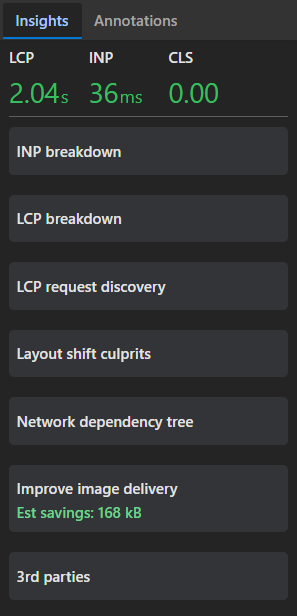
\includegraphics[width=0.55\textwidth]{Images/testing/devtool.png}
    \caption{Kết quả phân tích hiệu suất bằng Chrome DevTools}
    \label{fig:devtools-performance}
\end{figure}

\begin{table}[H]
\centering
\caption{Kết quả đo hiệu suất bằng Chrome DevTools}
\begin{tabularx}{\textwidth}{|p{0.18\textwidth}|p{0.18\textwidth}|X|}
\hline
\textbf{Chỉ số} & \textbf{Kết quả} & \textbf{Nhận xét} \\ \hline
LCP & 2.04s & Thời gian hiển thị nội dung lớn nhất ở mức chấp nhận được, tuy nhiên vẫn có thể tối ưu thêm bằng lazy loading và tối ưu ảnh. \\ \hline
INP & 36ms & Thời gian phản hồi tương tác rất tốt, thao tác click và nhập liệu không có độ trễ đáng kể. \\ \hline
CLS & 0.00 & Giao diện ổn định, không ghi nhận hiện tượng dịch chuyển bố cục trong quá trình tải trang. \\ \hline
\end{tabularx}
\end{table}

Kết quả quan sát cho thấy các trang chính đã có cơ chế phân trang hoặc tải dữ liệu theo nhu cầu. Feed, marketplace, notification, scheduled posts và các danh sách quản trị không tải toàn bộ dữ liệu cùng lúc mà gọi API theo trang hoặc theo bộ lọc. Những tài nguyên ảnh phụ thuộc nhiều vào dữ liệu upload và Cloudinary URL, do đó cần tiếp tục tối ưu kích thước ảnh, lazy loading và cache trình duyệt trong các phiên bản sau.

\subsection{Phân tích Lighthouse của Chrome DevTools}

Lighthouse được sử dụng để đánh giá tổng quan chất lượng frontend theo các nhóm chỉ số:

\begin{itemize}
    \item \textbf{Performance}: hiệu năng tải trang, thời gian render và khả năng phản hồi.
    \item \textbf{Accessibility}: khả năng truy cập, contrast, label của form, alt text cho hình ảnh.
    \item \textbf{Best Practices}: cấu hình bảo mật trình duyệt, HTTPS, lỗi console và sử dụng API web an toàn.
    \item \textbf{SEO}: thẻ meta cơ bản, title, mô tả và khả năng crawl với các trang public.
\end{itemize}

\begin{figure}[H]
    \centering
    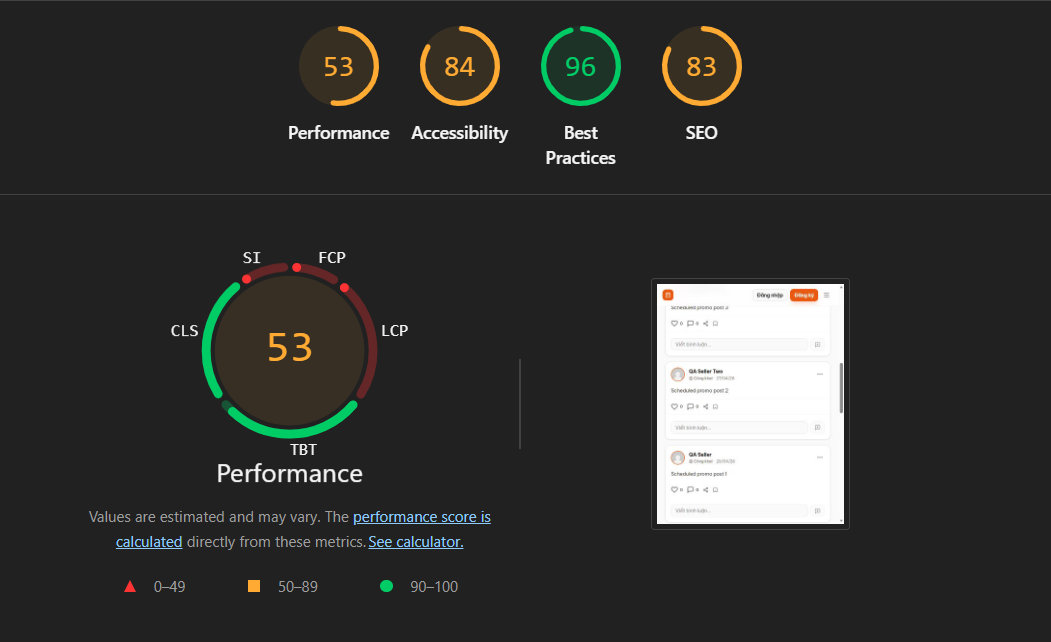
\includegraphics[width=0.95\textwidth]{Images/testing/lighthouse.png}
    \caption{Kết quả phân tích bằng Lighthouse}
    \label{fig:lighthouse-performance}
\end{figure}

\begin{table}[H]
\centering
\caption{Phân tích kết quả Lighthouse theo nhóm chỉ số}
\begin{tabularx}{\textwidth}{|p{0.18\textwidth}|p{0.12\textwidth}|X|p{0.25\textwidth}|}
\hline
\textbf{Nhóm chỉ số} & \textbf{Điểm} & \textbf{Nhận xét} & \textbf{Hướng cải thiện} \\ \hline
Performance & 53 & Điểm hiệu năng ở mức trung bình. Trang có nhiều component, dữ liệu động và media nên thời gian tải/render còn bị ảnh hưởng. & Tối ưu bundle, lazy load component, nén ảnh, dùng skeleton loading, cache hợp lý và giảm JavaScript không cần thiết. \\ \hline
Accessibility & 84 & Khả năng truy cập ở mức khá. Các form chính như login, register, OTP, checkout và seller form đã có label/placeholder cơ bản. & Rà soát thêm aria-label cho icon button, trạng thái lỗi form và contrast ở dark mode. \\ \hline
Best Practices & 96 & Điểm best practices tốt, cho thấy frontend và backend đã đáp ứng phần lớn khuyến nghị cơ bản về triển khai web. & Tiếp tục kiểm tra console warning, cấu hình HTTPS production và kiểm soát mixed content. \\ \hline
SEO & 83 & SEO ở mức khá đối với các trang public như feed, marketplace và product detail. & Bổ sung meta title/description động cho product detail, seller profile và post detail. \\ \hline
\end{tabularx}
\end{table}

Nhìn chung, kết quả kiểm thử hiệu suất cho thấy hệ thống đáp ứng được nhu cầu sử dụng trong phạm vi đồ án. Tuy nhiên, khi dữ liệu tăng lớn hoặc triển khai production với lượng truy cập cao, hệ thống cần tiếp tục được kiểm thử bằng các công cụ chuyên dụng hơn như k6, JMeter hoặc Artillery để đo throughput, latency theo percentiles và khả năng chịu tải của backend API.


